\chapter{Principi di Laser e Telemetria}
\label{capitolo1}
\thispagestyle{empty}

\textit{In questo Capitolo verranno richiamati i concetti fondamentali relativi al funzionamento delle sorgenti laser. Verranno quindi descritte le principali tipologie di sorgenti e le classi di sicurezza che ne regolamentano l'utilizzo. Successivamente, verr\'a esposto lo stato dell'arte dei misuratori ottici di distanza assoluta, ponendo particolare attenzione alle tecniche di misura a triangolazione, a tempo di volo e a onda continua. In conclusione, quest'ultime verranno messe a confronto con una tecnica alternativa, l'interferometria a retroiniezione, al fine di motivare l'utilizzo di tale tecnica per questo lavoro di Tesi.}

\section{Principi di funzionamento del laser}
LASER \'e l'acronimo di \emph{Light Amplification by Stimulated Emission of Radiation}, cio\'e amplificazione della luce mediante il fenomeno dell'emissione stimolata di radiazione~\cite{sveltolaser}. In generale, un laser \'e un dispositivo elettronico in grado di emettere un fascio di luce.
Un fascio di luce \'e un onda elettromagnetica costituita da particelle chiamate fotoni. Il fotone \'e il quanto di energia della radiazione elettromagnetica.

Il fascio di luce emesso da un dispositivo laser possiede tre caratteristiche principali:
\begin{enumerate}
	\item Coerenza
	\item Monocromaticit\'a
	\item Direzionalit\'a
\end{enumerate}

Per quanto riguarda la prima caratteristica ci si riferisce in particolare a due aspetti differenti: la coerenza spaziale e la coerenza temporale. La coerenza spaziale esprime la correlazione tra i valori che il campo elettromagnetico emesso assume in due punti diversi dello spazio, mentre per coerenza temporale si definisce la correlazione tra i valori che il campo elettromagnetico assume in due istanti di tempo diversi.
Un onda \'e coerente spaziale se esiste una differenza di fase costante tra due punti qualunque sul fronte d'onda. Mentre, la coerenza temporale \'e strettamente legata al tempo di coerenza. Esso \'e l'intervallo medio di tempo nel quale l'onda compir\'a un certo numero di oscillazioni prima di cambiare fase.

La seconda propriet\'a garantisce che tutti i fotoni generati per effetto dell'emissione stimolata risultino iso-frequenziali (aventi tutti la stessa frequenza). Essa \'e strettamente correlata alla coerenza temporale.

La terza e ultima propriet\'a, invece, afferma che la radiazione emessa dalla sorgente si propaga nello spazio in un'unica direzione ben definita con piccoli angoli di divergenza del fascio parallelo e perpendicolare, pi\'u precisamente, l'angolo solido sotteso da un fascio laser \'e estremamente piccolo. Essa \'e strettamente correlata alla coerenza spaziale.

Queste propriet\'a fondamentali di una sorgente laser sono dovute al principio di funzionamento stesso: l'emissione stimolata di radiazione.

\subsection{Emissione stimolata di radiazione}
Il fenomeno che permette il funzionamento del laser \'e l'emissione stimolata, per questo \'e importante capire di cosa si tratta e in che modo essa \'e differente dall'emissione spontanea. Per fare ci\'o \'e conveniente richiamare alcuni concetti di base.

Come accennato in precedenza, la propagazione della luce nello spazio si sviluppa tramite particelle dette fotoni (o quanti), aventi ciascuna una energia pari a:
\begin{equation}
E=h\nu
\end{equation}
dove $h= \SI{6.62e-34}{J.s}$ \'e la costante di Planck, mentre $\nu$ \'e la frequenza della radiazione. A sua volta la frequenza $\nu$ \'e in relazione alla lunghezza d'onda $\lambda$ tramite la relazione:
\begin{equation}
\nu= \frac{c}{\lambda}
\end{equation}
dove $c= \SI{2.99e8}{m.\per.s}$ rappresenta la velocit\'a della luce nel vuoto.

Un laser \'e un sistema ottico costituito da due specchi separati da un mezzo attivo, il quale pu\'o essere un solido, un liquido, un gas o un semiconduttore. Si consideri il mezzo attivo come un insieme di atomi (sistema atomico) e per semplicit\'a di trattazione si ipotizzi che il materiale attivo in questione, investito dalla radiazione, abbia due soli livelli energetici dotati rispettivamente di energia $E_{1}$ e $E_{2}$ con $E_{2}>E_{1}$. Definiamo lo stato ad energia inferiore $E_{1}$ come stato fondamentale e lo stato ad energia superiore $E_{2}$ come stato eccitato.
\begin{figure}
  \begin{center}
    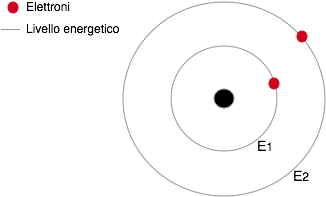
\includegraphics[scale=0.7]{cap1/atomico2liv}
    \caption{Sistema atomico composto da due livelli}
    \label{atomico2liv}
  \end{center}
\end{figure}

Quando la luce investe un materiale, si possono verificare due differenti tipi di transizione:
\begin{itemize}
	\item \emph{Assorbimento}: Quando il fascio di luce investe un materiale, parte dell'energia posseduta dal fascio viene ceduta. L'assorbimento consiste nel cedere, da parte del fotone, la propria energia al sistema atomico permettendo ad un singolo elettrone di passare da uno stato fondamentale $E_{1}$ ad uno stato eccitato $E_{2}$.
	\item \emph{Emissione}: Il sistema atomico cede energia al campo, in questo caso si possono avere due possibili scenari:
	\begin{itemize}
		\item \emph{Spontanea}: L'emissione spontanea si verifica quando un elettrone torna dal livello $E_{2}$ al livello $E_{1}$, provocando l'emissione di un fotone, senza nessun campo di radiazione incidente su di esso. Essa viene definita anche emissione incoerente: l'energia viene emessa con fase e direzione casuale.
		\item \emph{Stimolata}: L'emissione stimolata, invece, si ottiene quando un fotone incidente causa la discesa di un elettrone dal livello $E_{2}$ al livello $E_{1}$ ottenendo così due fotoni alla stessa frequenza. Quindi, in breve, un fotone colpisce l'atomo e due fotoni lo lasciano. Essa viene definita anche emissione coerente: l'energia viene emessa con la stessa fase, frequenza e direzione.
	\end{itemize} 
\end{itemize}
\begin{figure}
  \begin{center}
    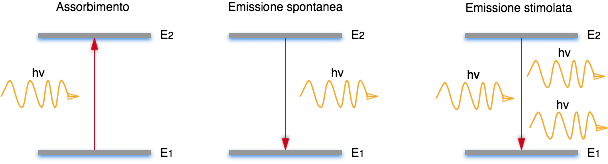
\includegraphics[scale=0.6]{cap1/funzatomoecc}
    \caption{Schema di funzionamento di un atomo eccitato: assorbimento, emissione spontanea ed emissione stimolata}
    \label{funzatomoecc}
  \end{center}
\end{figure}
L'importanza dell'emissione stimolata sta nel fatto che essendo prodotti due fotoni iso-frequenziali, di fatto avviene un'amplificazione ottica, la quale consente il funzionamento del sistema laser.

Per comprendere i meccanismi che regolano lo scambio di energia tra la radiazione ed il sistema atomico, è necessario introdurre la statistica di Boltzmann~\cite{kasap2012optoelectronics}. Attraverso tale statistica \'e possibile definire la popolazione, in termini di densit\'a, di un livello energetico all'equilibrio termico mediante la seguente relazione:
\begin{equation}
  N=N_0e^{{-\frac{E}{kT}}}
\end{equation}
dove $N_0$ \'e la popolazione iniziale in un dato livello energetico e $k=1.38\cdot10^{-23}\frac{J}{K}$\'e la costante di Boltzmann.
 
 Indicando, quindi, con $N_1$ e $N_2$ il numero di atomi per unit\'a di volume (popolazione atomica) per i rispettivi livelli $E_1$ e $E_2$, possiamo ricavare il rapporto tra il numero di atomi nello stato fondamentale e quello nello stato eccitato, all'equilibrio termodinamico alla temperatura $T$, tramite la seguente equazione:
\begin{equation}
	\frac{N_2}{N_1}=e^{-\frac{\Delta E}{kT}} 
	\label{rappboltz}
\end{equation}
dove $\Delta E = E_2 - E_1$.

La condizione necessaria per avere emissione stimolata \'e l'inversione di popolazione tra i due livelli energetici, ovvero, il numero di atomi presenti nel livello eccitato deve essere maggiore di quello fondamentale ($N_2 > N_1$).

In un sistema a due livelli questa condizione non \'e realizzabile poich\'e, come possiamo osservare dall'equazione \ref{rappboltz} a causa della presenza dell'esponenziale negativo, $N_1$ risulta sempre maggiore di $N_2$, ovvero gli atomi a energia minima sono maggiori rispetto a quelli eccitati. 
\'E evidente dunque che, per avere una maggior probabilit\'a di emissione rispetto all'assorbimento, sia necessaria un'inversione di popolazione, ovvero $N_2 > N_1$.

Per ottenere la condizione di inversione di popolazione \'e quindi necessario l'utilizzo di un sistema atomico con almeno tre livelli energetici.

\subsection{Inversione di popolazione}
\begin{figure}
  \begin{center}
    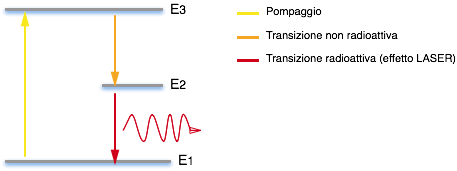
\includegraphics[scale=0.6]{cap1/sistema3liv}
    \caption{Sistema atomico a tre livelli energetici}
    \label{sistema3liv}
  \end{center}
\end{figure}
L'idea di base dell'inversione di popolazione consiste nello sfruttare i diversi tempi di vita medi dei differenti stati energetici.

Considerando un sistema ad esattamente tre livelli energetici ($E_1$, $E_2$ e $E_3$) schematizzato in Figura \ref{sistema3liv}, si sottopone il sistema atomico ad una radiazione luminosa di frequenza $\nu_{31}$, corrispondente al gap energetico $E_3-E_1$, in modo tale che gli elettroni dallo stato $E_1$ si eccitino raggiungendo lo stato instabile $E_3$. Questa prima fase è chiamata \emph{pompaggio}.

Successivamente si manifesta un decadimento dallo stato instabile $E_3$ allo stato $E_2$ in tempi molto rapidi e privi di emissione spontanea. Solitamente l'energia rilasciata viene trasferita sotto forma di moto vibrazionale al materiale circostante e non come fotone emesso.

Dal livello $E_2$ si verifica l'emissione laser alla frequenza $\nu_{21}$ e la conseguente regressione dal livello $E_2$ al livello $E_1$. La condizione necessaria, sui tempi di vita medi, per il funzionamento del laser è $\tau_{32} << \tau_{21}$, ovvero che il decadimento da $E_3$ a $E_2$ sia pi\'u rapido di quello da $E_2$ a $E_1$. Tale condizione permette di avere inversione di popolazione, ovvero $N_2 > N_1$, cos\'i da poter innescare l'amplificazione ottica e, quindi, l'effetto laser alla frequenza $\nu_{21}$.

Questo metodo \'e inefficiente perch\'e richiede un pompaggio elevato: \'e necessario fornire un numero elevato di elettroni al livello $E_3$ in modo tale che possa donarli al livello $E_2$ permettendo cos\'i l'inversione di popolazione.
\begin{figure}
  \begin{center}
    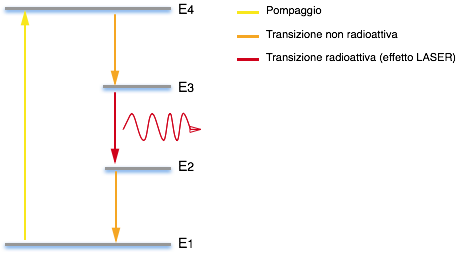
\includegraphics[scale=0.6]{cap1/sistema4liv}
    \caption{Sistema atomico a quattro livelli energetici}
    \label{sistema4liv}
  \end{center}
\end{figure}
Un struttura pi\'u efficiente \'e quella a quattro livelli schematizzata in Figura \ref{sistema4liv}. In questa disposizione, il pompaggio degli elettroni avviene da $E_1$ a $E_4$ a cui segue una transizione rapida e senza radiazione verso $E_3$ che consente di popolare il livello energetico. A questo punto avviene la transizione lenta e l'emissione tramite azione laser. Infine avviene una rapida transizione da $E_2$ allo stato fondamentale $E_1$.

A differenza della struttura a tre livelli, questa ha il vantaggio di avere il livello $E_3$ popolato mentre il livello $E_2$ vuoto ($N_2=0$), in quanto gli elettroni decadono rapidamente dallo stato $E_2$ allo stato $E_1$, aiutando a conservare l'inversione di popolazione $N_3 >> N_2$. 
				
Oltre al meccanismo appena descritto, altre caratteristiche risultano cruciali nel funzionamento del laser: la cavit\'a ottica e il materiale attivo.

\subsection{Cavit\'a ottica e materiale attivo}
Nel paragrafo precedente abbiamo visto come realizzare un materiale amplificatore, che sfrutta l'inversione di popolazione nei livelli energetici. Per generare il fascio laser \'e necessario, per\'o, inserire il materiale attivo all'interno di una cavit\'a ottica.
\begin{figure}  
  \begin{center}
    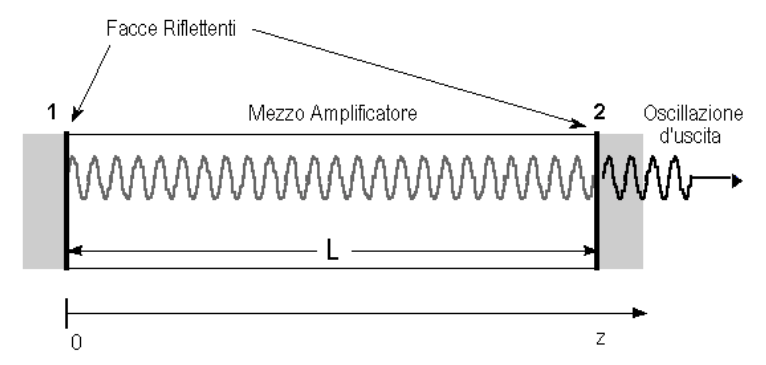
\includegraphics[scale=0.4]{cap1/cavitaottica}
    \caption{Cavit\'a di Fabry-Perot}
    \label{cavitaottica}
  \end{center}
\end{figure}
Una semplice cavit\'a ottica può essere rappresentata dalla cavit\'a a specchi piani e paralleli, nota anche come cavit\'a di Fabry-Perot, mostrata in Figura \ref{cavitaottica}. 
\begin{figure}  
  \begin{center}
    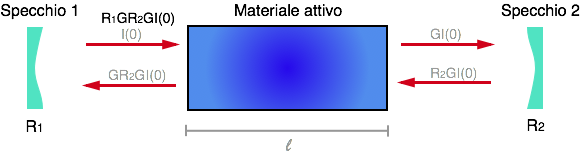
\includegraphics[scale=0.6]{cap1/roundtrip}
    \caption{Schema del Roundtrip ottico nella cavit\'a ottica}
    \label{roundtrip}
  \end{center}
\end{figure}
Il fascio di luce viaggia avanti-indietro riflettendosi negli specchi e amplificandosi nel passaggio all'interno del materiale attivo. Il fascio laser in uscita si ottiene rendendo uno dei due specchi della cavit\'a ottica parzialmente trasparente, in modo tale che parte della radiazione esca dalla cavit\'a.

Per definire il guadagno ottico del materiale attivo \'e necessario introdurre per\'o alcuni concetti preliminari. Indicando con $I$ l'intensità luminosa, definiamo l'intensità della luce all'interno della cavit\'a ottica con la seguente relazione:
\begin{equation}
I(l)=I(0)e^{\sigma(N_2-N_1)l}
\end{equation}
dove $\sigma$ \'e la la \textit{cross section} di emissione e $l$ \'e la lunghezza della cavit\'a ottica.
\begin{figure}  
  \begin{center}
    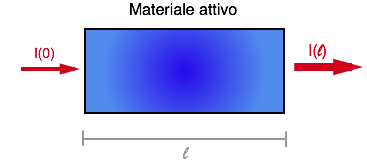
\includegraphics[scale=0.6]{cap1/propagazione}
    \caption{Propagazione della radiazione all'interno della cavità laser}
    \label{propagazione}
  \end{center}
\end{figure}
Possiamo definire il guadagno ottico del mezzo attivo come:
\begin{equation}
  G=\frac{I(l)}{I(0)}=e^{\sigma(N_2-N_1)l}
\end{equation}
sulla quale graveranno le limitazioni dovute alle perdite del materiale e alla perdita utile di potenza dovuta al laser uscente.

La cavità ottica e il mezzo attivo formano quindi un oscillatore ottico, ossia un amplificatore che viene retro-azionato positivamente attraverso specchi riflettenti posti ai lati del materiale attivo. Quindi, per avere un'azione laser è necessario raggiungere una situazione in cui il guadagno di amplificazione sia tale da compensare tutte le perdite presenti. 

Considerando come perdite solamente la riflettività parziale degli specchi $R_1$ e $R_2$, l'oscillazione ottica si innesca quando il guadagno del materiale attivo supera le perdite della cavità in un giro completo, o \textit{round trip}:
\begin{equation}
  G^2=\frac{1}{R_1R_2}
\end{equation}
Quest'ultimo è chiamato guadagno critico o inversione critica.

\section{Laser a semiconduttore}

%%TODO Cap 1: Laser a semiconduttore








 







